% questions.tex —— 2002 年·上海卷·文科 · 题目内容片段（无答案）
% 由 tools/generate_projects.py 依来源总账自 2002/2002_数学真题_上海文_试题.md 生成，勿手改（改源 MD 后重跑）


\gkpart{数学}

\begin{gktip}
\textbf{来源说明}：本题面依据固定源 PDF 两页题面逐题转录，原卷印刷页码 110–111。固定源不附答案，答案和解析均由本库独立复算。

\textbf{图形说明}：第 13、15、16、17 题的原卷图形关系重绘为 TikZ/PGFPlots 矢量图。图形标记所指的 PNG 不随仓库保存。
\end{gktip}

\gkpart{一、填空题}

\begin{question}
\gkti{1}若 $z\in\mathbb C$，$(3+z)i=1$（$i$ 为虚数单位），则 $z=$\gkblank{}。

\end{question}
\begin{question}
\gkti{2}已知向量 $\vec a$ 和 $\vec b$ 的夹角为 $120^\circ$，且 $|\vec a|=2$，$|\vec b|=5$，则

\nopagebreak[4]
\[
(2\vec a-\vec b)\cdot\vec a=
\]

\gkblank{}。

\end{question}
\begin{question}
\gkti{3}方程

\nopagebreak[4]
\[
\log_3(1-2\cdot3^x)=2x+1
\]

的解 $x=$\gkblank{}。

\end{question}
\begin{question}
\gkti{4}若正四棱锥的底面边长为 $2\sqrt3\text{ cm}$，体积为 $4\text{ cm}^3$，则它的侧面与底面所成的二面角的大小是\gkblank{}。

\end{question}
\begin{question}
\gkti{5}在二项式 $(1+3x)^n$ 和 $(2x+5)^n$ 的展开式中，各项系数之和分别记为 $a_n\text{、}b_n$，$n$ 是正整数，则

\nopagebreak[4]
\[
\lim_{n\to\infty}\frac{a_n-2b_n}{3a_n-4b_n}
\]

等于\gkblank{}。

\end{question}
\begin{question}
\gkti{6}已知圆

\nopagebreak[4]
\[
x^2+(y-1)^2=1
\]

和圆外一点 $P(-2,0)$，过点 $P$ 作圆的切线，则两条切线夹角的正切值是\gkblank{}。

\end{question}
\begin{question}
\gkti{7}在某次花样滑冰比赛中，发生裁判受贿事件，竞赛委员会决定将裁判由原来的 9 名增至 14 名，但只任取其中 7 名裁判的评分作为有效分。若 14 名裁判中有 2 人受贿，则有效分中没有受贿裁判的评分的概率是\gkblank{}。（结果用数值表示）

\end{question}
\begin{question}
\gkti{8}抛物线

\nopagebreak[4]
\[
(y-1)^2=4(x-1)
\]

的焦点坐标是\gkblank{}。

\end{question}
\begin{question}
\gkti{9}某工程由下列工序组成，则工程总时数为\gkblank{}天。

\begin{center}
\begin{tabular}{lrrrrrr}
\toprule
工序 & $a$ & $b$ & $c$ & $d$ & $e$ & $f$ \\
\midrule
紧前工序 & — & — & $a\text{、}b$ & $c$ & $c$ & $d\text{、}e$ \\
工时数（天） & 2 & 3 & 2 & 5 & 4 & 1 \\
\bottomrule
\end{tabular}
\end{center}

\end{question}
\begin{question}
\gkti{10}设函数 $f(x)=\sin2x$，若 $f(x+t)$ 是偶函数，则 $t$ 的一个可能值是\gkblank{}。

\end{question}
\begin{question}
\gkti{11}若数列 $\{a_n\}$ 中，$a_1=3$，且 $a_{n+1}=a_n^2$（$n$ 是正整数），则数列的通项

\nopagebreak[4]
\[
a_n=
\]

\gkblank{}。

\end{question}
\begin{question}
\gkti{12}已知函数 $y=f(x)$（定义域为 $D$，值域为 $A$）有反函数 $y=f^{-1}(x)$，则方程 $f(x)=0$ 有解 $x=a$，且 $f(x)>x$（$x\in D$）的充要条件是 $y=f^{-1}(x)$ 满足\gkblank{}。

\end{question}
\gkpart{二、选择题}

\Needspace{0.4\textheight}
\begin{question}
\gkti{13}如图，与复平面中的阴影部分（含边界）对应的复数集合是\mbox{（　　）}
\nopagebreak[4]
\begin{center}% 2002 年上海文科第 13 题：复平面阴影区域
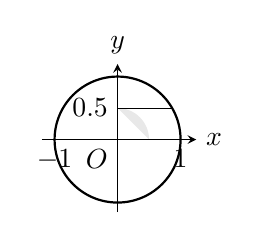
\begin{tikzpicture}[scale=0.8, >=stealth]
  \fill[gray!18] (0,0.5) arc (90:0:0.5) -- (0,0.5) -- cycle;
  \draw[thick] (0,0) circle (1);
  \draw[->] (-1.2,0)--(1.25,0) node[right] {$x$};
  \draw[->] (0,-1.15)--(0,1.2) node[above] {$y$};
  \draw (0,0.5)--(0.866,0.5);
  \node[left] at (0,0.5) {$0.5$};
  \node[below left] at (0,0) {$O$};
  \node[below] at (-1,0) {$-1$};
  \node[below] at (1,0) {$1$};
\end{tikzpicture}
\end{center}
\nopagebreak[4]
（A）$\{z\mid |z|=1,\ \operatorname{Re}z\ge\dfrac12,\ z\in\mathbb C\}$

（B）$\{z\mid |z|\le1,\ \operatorname{Re}z\ge\dfrac12,\ z\in\mathbb C\}$

（C）$\{z\mid |z|=1,\ \operatorname{Im}z\ge\dfrac12,\ z\in\mathbb C\}$

（D）$\{z\mid |z|\le1,\ \operatorname{Im}z\ge\dfrac12,\ z\in\mathbb C\}$

\end{question}
\begin{question}
\gkti{14}已知直线 $l\text{、}m$，平面 $\alpha\text{、}\beta$，且 $l\perp\alpha$，$m\subset\beta$，给出下列四个命题：

① 若 $\alpha\parallel\beta$，$l\perp m$；② $l\perp m$，$\alpha\parallel\beta$；③ 若 $\alpha\perp\beta$，则 $l\parallel m$；④ 若 $l\parallel m$，$\alpha\perp\beta$。

其中正确命题的个数是\mbox{（　　）}

（A）1 个　　（B）2 个　　（C）3 个　　（D）4 个

\Needspace{0.4\textheight}
\end{question}
\begin{question}
\gkti{15}函数 $y=x+\sin|x|$，$x\in[-\pi,\pi]$ 的大致图象是\mbox{（　　）}
\nopagebreak[4]
\begin{center}% 2002 年上海文科第 15 题：函数图象选项示意
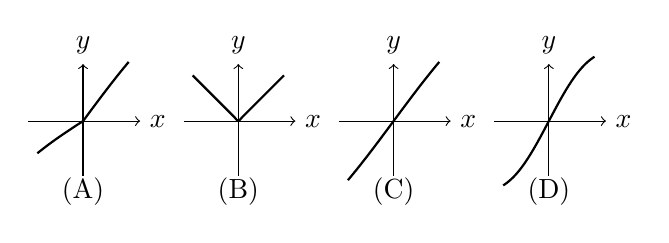
\begin{tikzpicture}[scale=0.58]
  \foreach \shift/\lab in {0/A,3.4/B,6.8/C,10.2/D} {
    \begin{scope}[xshift=\shift cm]
      \draw[->] (-1.2,0)--(1.25,0) node[right] {$x$};
      \draw[->] (0,-1.2)--(0,1.25) node[above] {$y$};
      \node at (0,-1.55) {(\lab)};
    \end{scope}
  }
  \draw[thick, domain=-1:1, smooth] plot ({\x},{\x+0.35*sin(deg(abs(\x)))});
  \draw[thick, domain=-1:1, smooth, xshift=3.4cm] plot ({\x},{abs(\x)});
  \draw[thick, domain=-1:1, smooth, xshift=6.8cm] plot ({\x},{\x+0.35*sin(deg(\x))});
  \draw[thick, domain=-1:1, smooth, xshift=10.2cm] plot ({\x},{\x+0.45*sin(deg(2*\x))});
\end{tikzpicture}
\end{center}
\nopagebreak[4]
（A）　　（B）　　（C）　　（D）

\Needspace{0.4\textheight}
\end{question}
\begin{question}
\gkti{16}一般地，家庭用电量（千瓦时）与气温（摄氏度）有一定的关系。图（1）表示某年 12 个月中每月的平均气温，图（2）表示某家庭在这年 12 个月中每月的用电量。根据这些信息，以下关于该家庭用电量与气温间关系的叙述中，正确的是\mbox{（　　）}
\nopagebreak[4]
\begin{center}% 2002 年上海文科第 16 题：月度气温与用电量统计图
\begin{tikzpicture}[x=0.34cm,y=0.035cm]
  \draw[->] (0,0)--(13,0) node[right] {月份};
  \draw[->] (0,0)--(0,32) node[above] {气温};
  \foreach \x/\h in {1/3,2/8,3/14,4/18,5/23,6/27,7/28,8/24,9/17,10/12,11/5,12/2}
    \draw[fill=gray!15] (\x-0.42,0) rectangle (\x+0.42,\h);
  \begin{scope}[xshift=6cm,yshift=0cm]
    \draw[->] (0,0)--(13,0) node[right] {月份};
    \draw[->] (0,0)--(0,130) node[above] {用电量};
    \foreach \x/\h in {1/115,2/120,3/95,4/80,5/75,6/80,7/110,8/120,9/95,10/75,11/85,12/100}
      \draw[fill=gray!15] (\x-0.42,0) rectangle (\x+0.42,\h);
  \end{scope}
\end{tikzpicture}
\end{center}
\nopagebreak[4]
（A）气温最高时，用电量最多

（B）气温最低时，用电量最少

（C）当气温大于某一值时，用电量随气温增高而增加

（D）当气温小于某一值时，用电量随气温降低而增加

\end{question}
\gkpart{三、解答题}

\Needspace{0.4\textheight}
\begin{question}
\gkti{17}如图，在直三棱柱 $ABO-A'B'O'$ 中，$OO'=4$，$OA=4$，$OB=3$，$\angle AOB=90^\circ$，$D$ 是线段 $A'B'$ 的中点，$P$ 是侧棱 $BB'$ 上的一点。若 $OP\perp BD$，求 $OP$ 与底面 $AOB$ 所成角的大小。（结果用反三角函数值表示）
\nopagebreak[4]
\begin{center}% 2002 年上海文科第 17 题：直三棱柱空间图
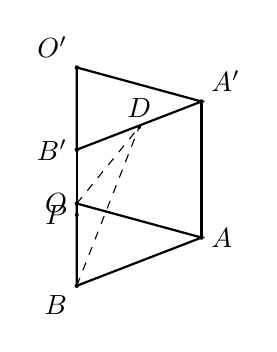
\begin{tikzpicture}[>=stealth, scale=0.72]
  \coordinate (O) at (0,0);
  \coordinate (A) at (2.2,-0.6);
  \coordinate (B) at (0,-1.45);
  \coordinate (Op) at (0,2.4);
  \coordinate (Ap) at (2.2,1.8);
  \coordinate (Bp) at (0,0.95);
  \coordinate (D) at (1.1,1.35);
  \coordinate (P) at (0,-0.2);
  \draw[thick] (O)--(A)--(B)--cycle;
  \draw[thick] (Op)--(Ap)--(Bp)--cycle;
  \draw[thick] (O)--(Op) (A)--(Ap) (B)--(Bp);
  \draw[dashed] (O)--(D) (B)--(D);
  \draw[thick] (O)--(P);
  \fill (O) circle (1.1pt) node[left] {$O$};
  \fill (A) circle (1.1pt) node[right] {$A$};
  \fill (B) circle (1.1pt) node[below left] {$B$};
  \fill (Op) circle (1.1pt) node[above left] {$O'$};
  \fill (Ap) circle (1.1pt) node[above right] {$A'$};
  \fill (Bp) circle (1.1pt) node[left] {$B'$};
  \fill (D) circle (1.0pt) node[above] {$D$};
  \fill (P) circle (1.0pt) node[left] {$P$};
\end{tikzpicture}
\end{center}
\nopagebreak[4]
\end{question}
\begin{question}
\gkti{18}已知点 $A(-\sqrt3,0)$ 和 $B(\sqrt3,0)$，动点 $C$ 到 $A\text{、}B$ 两点的距离之差的绝对值为 2，点 $C$ 的轨迹与直线 $y=x-2$ 交于 $D\text{、}E$ 两点，求线段 $DE$ 的长。

\end{question}
\begin{question}
\gkti{19}已知函数

\nopagebreak[4]
\[
f(x)=x^2+2ax+2,\qquad x\in[-5,5].
\]

（1） 当 $a=-1$ 时，求函数 $f(x)$ 的最大值与最小值。

（2） 求实数 $a$ 的取值范围，使 $y=f(x)$ 在区间 $[-5,5]$ 上是单调函数。

\end{question}
\begin{question}
\gkti{20}某商场在促销期间规定：商场内所有商品按标价的 80\% 出售，同时，当顾客在该商场内消费满一定金额后，按如下方案获得相应金额的奖券：

\begin{center}
\begin{tabular}{lrrrrr}
\toprule
消费金额的范围 & $[200,400)$ & $[400,500)$ & $[500,700)$ & $[700,900)$ & $\cdots$ \\
\midrule
获得奖券的金额 & 30 & 60 & 100 & 130 & $\cdots$ \\
\bottomrule
\end{tabular}
\end{center}

购买商品得到的优惠额为折扣额与奖券金额之和。设购买商品得到的优惠率为优惠额与商品标价之比，试问：

（1） 若购买一件标价为 1000 元的商品，顾客得到的优惠率是多少？

（2） 对于标价在 $[500,800]$ 元内的商品，顾客购买标价为多少元的商品，可得到不小于 $\dfrac13$ 的优惠率？

\end{question}
\begin{question}
\gkti{21}已知函数 $f(x)=a\cdot b^x$ 的图象过点 $A(4,\dfrac14)$ 和 $B(5,1)$。

（1） 求函数 $f(x)$ 的解析式；

（2） 记 $a_n=\log_2f(n)$，$n$ 是正整数，$S_n$ 是数列 $\{a_n\}$ 的前 $n$ 项和，解关于 $n$ 的不等式 $a_nS_n\le0$；

（3） 对于（2）中的 $a_n$ 与 $S_n$，整数 96 是否为数列 $\{a_nS_n\}$ 中的项？若是，则求出相应的项数；若不是，则说明理由。

\end{question}
\begin{question}
\gkti{22}规定

\nopagebreak[4]
\[
C_x^m=\frac{x(x-1)\cdots(x-m+1)}{m!},
\]

其中 $x\in\mathbb R$，$m$ 是正整数，且 $C_0^x=1$。这是组合数 $C_n^m$（$n\text{、}m$ 是正整数，且 $m\le n$）的一种推广。

（1） 求 $C_{-15}^3$ 的值；

（2） 设 $x>0$，当 $x$ 为何值时，$\dfrac{C_x^3}{(C_x^1)^2}$ 取得最小值？

（3） 组合数的两个性质：① $C_n^m=C_n^{n-m}$；② $C_n^m+C_n^{m-1}=C_{n+1}^m$ 是否都能推广到 $C_x^m$（$x\in\mathbb R$，$m$ 是正整数）的情形？若能推广，则写出推广的形式并给出证明；若不能，则说明理由。

\end{question}